\begin{itemize}
  \item Strukturoptimierung
  \item Parameteroptimierung
  \item Verifikation
\end{itemize}
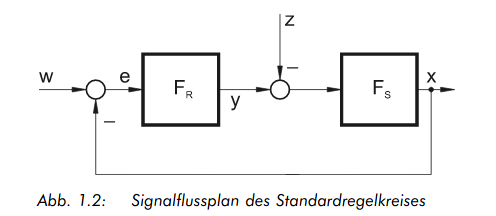
\includegraphics[scale= 0.5]{themen/pict/standardregelkreis.png}

\subsubsection{Enstellregel nach Ziegler/Nichols}
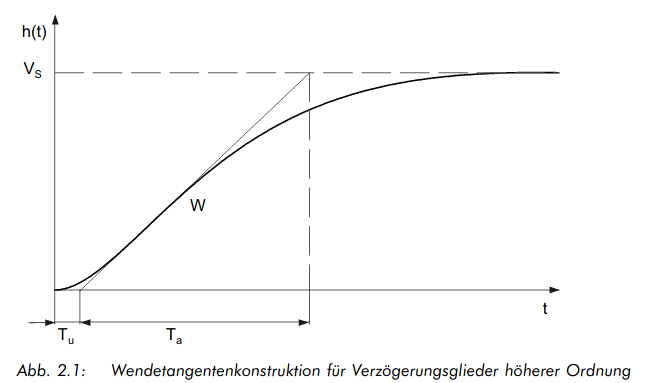
\includegraphics[scale= 0.5]{themen/pict/wendetangente.png}

Zur Messung an der Stabilitätsgrenze sind folgende Schritte nötig:\\
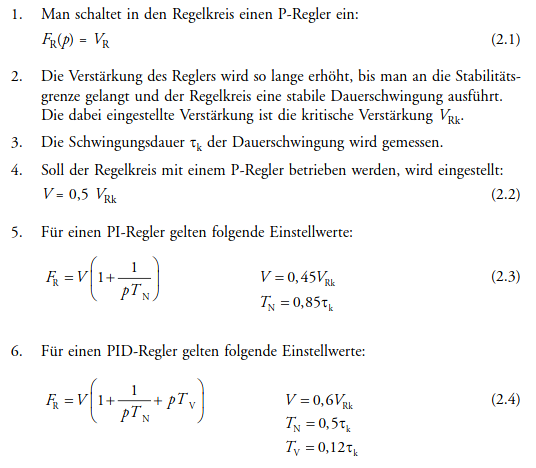
\includegraphics[scale= 0.5]{themen/pict/variante1-ziegler.png}

Wenn die Messung an der Stabilitätsgrenze nich möglich ist, wird die Sprungantwort gemessen. \\
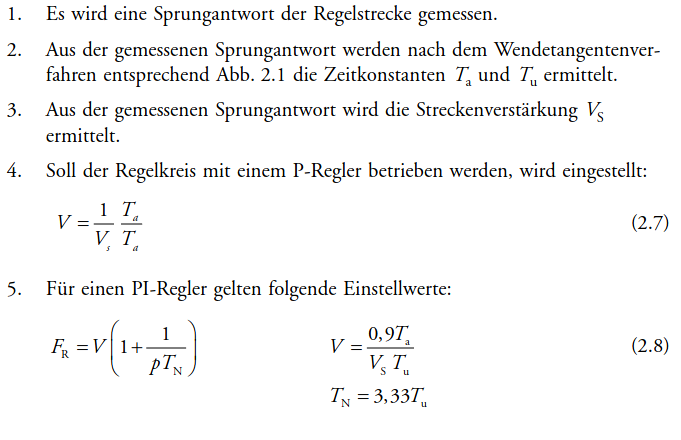
\includegraphics[scale= 0.5]{themen/pict/variante2.png}\\
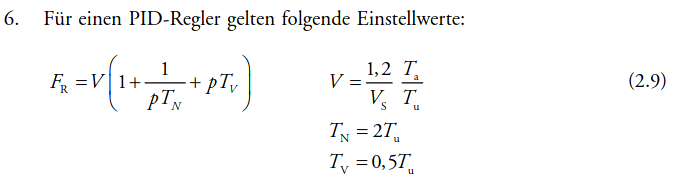
\includegraphics[scale= 0.5]{themen/pict/variante2-2.png}

\subsubsection{Einstellregel nach Chien/Hrones/Reswick}
unterscheidet zwischen Einstellung nach optimalem Führungsverhalten oder Störverhalten, jeweils ohne und mit $20\%$ Überschwingung.

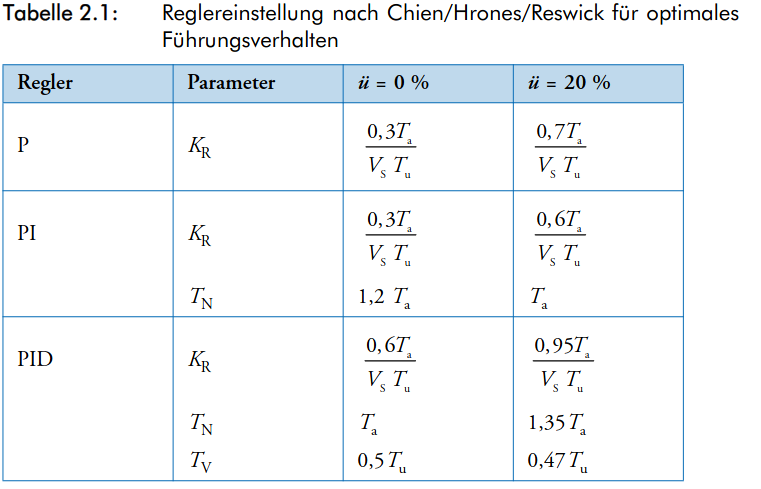
\includegraphics[scale= 0.5]{themen/pict/chien-fuehrung.png}\\

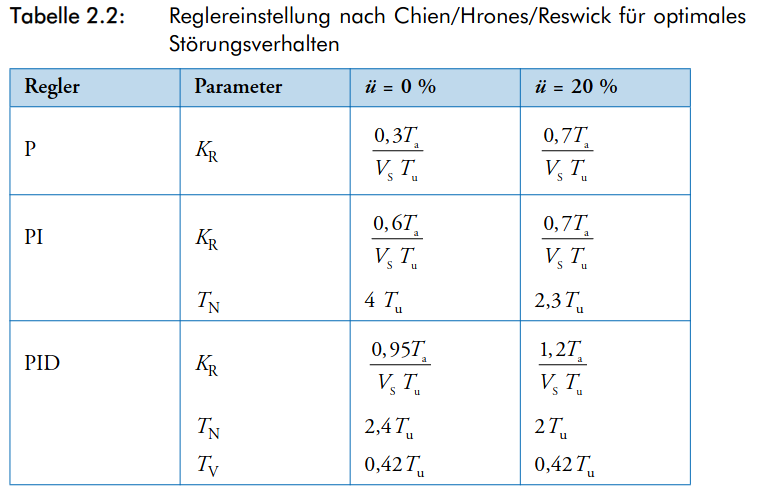
\includegraphics[scale= 0.5]{themen/pict/chien-stoerung.png}

Einstellwerte sind für ideale PID-Regler. Um sie realisierbar zu machen braucht es noch ein Verzögerungsglied.
Zeitkonstante $T_d = 3 \dots 50 T_v$. Experimentell bestimmt, beginnend bei $T_d = 4 T_v$

\subsubsection{Quadratisches Optimum }

 \begin{minipage}{0.45\textwidth}
  $\frac{dISE_3}{dV} = \frac{1}{2}\frac{a(bV - cV^2)-(aV+b)(b-2cV)}{(bV-cV^2)^2} = 0 $ \\
 $ V^2 + 2\cdot \frac{b}{a}\cdot V - \frac{b^2}{ac} = 0$
 aufgeläst ergibt sich:
 $ T_0 = V_s \cdot \frac{(T_1+T_2)\sqrt{T_1T_2}+T_1T_2}{T_1+T_2}$


 Mit zusätzlichem Verzögerungsglied wird Führungsverhalten verbessert (weniger Überschwingen)\\
 $F_V(p) = \frac{1}{1+pT_V} $ \\
 mit $T_{VQO} = 1,2 T_{\Sigma}$
 \end{minipage}
 \begin{minipage}{0.45\textwidth}

\legende{Ziel: Quadratische Regelfläche ISE wird \\minimal, allerdings großer Rechenaufwand\\}
 \legende{

 $\frac{dISE_3}{dV}$ & Ableitung  nach V  & & \\

 }
 \end{minipage}

\subsubsection{Betragsoptimum}
\begin{minipage}{0.45\textwidth}

vereinfachte Regelstrecke\\
$F_s = \frac{V_s}{\prod_{i=1}^k (1+pT_i)(1+pT_{\Sigma})}$\\
PID-Regler:\\
$F_R=\frac{\prod_{s=1}^r(1+pT_{RS})}{pT_0}$\\
offener Kreis ist damit:\\
$ F_0 = \frac{V_s \cdot \prod_{s=1}^r(1+pT_{RS})}{\prod_{i=1}^k (1+pT_i)(1+pT_{\Sigma})\cdot pT_0  }$
\end{minipage}
\begin{minipage}{0.45\textwidth}

\legende{
einfache, übersichtliche Einstellregeln\\ für Standardregelkreis\\

geeignet zur Ausregelung von Störgrößen,\\ die am Ausgang der Regelstrecke angreifen.


}
\end{minipage}


\textbf{Schritte zum Betragsoptimum:} \\
\begin{enumerate}
  \item Anzahl der Zählerzeitkonstanten des Reglers ist gleid der Anzahl k der großen Zeitkonstanten der Regelstrecke.
  \item Je eine Zählerzeitkonstante des REglers sei einer der großen Zeitkonstaten der Strecke gleich. $T_{Rs} = T_i $
  \item Einstellregel für die Integrierzeitkonstante:\\
  $T_0 = 2T_{\Sigma} \cdot V_S$
\end{enumerate}


Damit folgt: typische Übertragungsfunktion für den offenen Kreis
$F_o = \frac{1}{p2T_{\Sigma}(1+pT_{\Sigma})}$\\
Führungsverhalten geschlossener Kreis:
$F_w = \frac{1}{1+p2T_{\Sigma}(1+pT_{\Sigma})}$

typische Werte:\\
$\omega_d \approx \frac{1}{2T_{\Sigma}}$\\
$\gamma = 65,5 ^{\circ}$ (Aplitudengang)\\
$\gamma = 63 ^{\circ}$ (Asyptotenzug)\\

$ T_an \approx 5 T_{\Sigma}$; ü $\approx 5 \%$

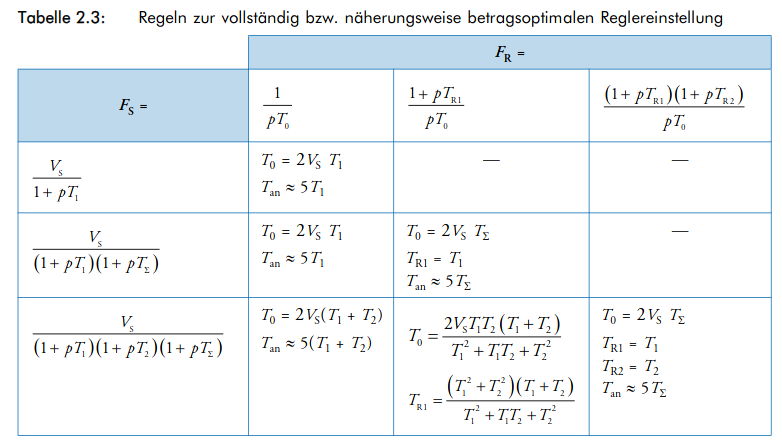
\includegraphics[scale = 0.5]{themen/pict/betragsoptimal.png}

\subsubsection{Symmetrisches Optimum, Einstellregel nach Kessler}


\begin{minipage}{0.45\textwidth}
  Einstellregeln PI-Regler:\\
  \mainformular{$ T_R = 4 T_{\Sigma}$ ; \\
  $ T_0 = 2V_S \frac{T_{\Sigma}T_R}{T_S} = 8V_S\frac{T_{\Sigma}^2}{T_s}$ }\\
  Einstellregel PID-Regler:\\
  \mainformular{$F_R= \frac{(1+pT_R)^2}{pT_0}$ ; \\
  $T_R = 8 T_{\Sigma}$ ; \\
  $T_0 = \frac{128T_{\Sigma}^3 V_S}{T_2T_3}$}
\end{minipage}
\begin{minipage}{0.45\textwidth}

\legende{
Anwendung in elektrischer Antriebstechnik
}
\end{minipage}


\subsubsection{Stochastisches Optimum}

\begin{minipage}{0.45\textwidth}
  \mainformular{$T_R = T_S$; $T_0 = \frac{1}{2} V_S T_{\Sigma}$}\\
  $\omega_d = \frac{\sqrt{2}}{T_{\Sigma}}$; $ \gamma = 35^\circ$

  Mit zusätzlichem Verzögerungsglied wird Führungsverhalten verbessert (weniger Überschwingen)\\
  $F_V(p) = \frac{1}{1+pT_V} $ \\
  mit $T_{VStO} = 1,2 T_{\Sigma}$
\end{minipage}
\begin{minipage}{0.45\textwidth}
\legende{
Verbesserung des Störverhaltens\\
Erhöhung der Reglergeschwindigkeit
}
\end{minipage}


\subsubsection{Einstellregel nach Naslin}
\begin{minipage}{0.45\textwidth}
Sei $F_w(p) = \frac{b_0}{a_0+a_1p+a_2p^2} = \frac{\frac{b_0}{a_0}}{1+\frac{a_1}{a_0}p+\frac{a_2}{a_0}p^2}$

Übertragungsfunktion des Schwingungsglieds: \\
$F_s(p)= \frac{1}{1+p2DT_0 + p^2T_0^2}$

Koeffizientenvergleich:
$4D^2 = \frac{a_1^2}{a_0a_2}$

und allg:
$\alpha = \frac{a_i^2}{a_{i-1} a_{i+1}}$


\end{minipage}
\begin{minipage}{0.45\textwidth}
\legende{
anwendbar, wenn Übertragungsfunktion\\ der Strecke bekannt\\
günstiges Führungsverhalten aber ohne\\ kurze Ausregelzeiten\\
nur für Zählerpolynom nullter Ordnung\\ und geradzahliges Nennenpolynom
}
\legende{günstige Verhältnisse: $1,5 \leq \alpha \leq 2,5$}
\end{minipage}
